% Compile with pdfLaTeX. No BibTeX or external theme is required.
% 15 main slides, approximately 18 minutes, plus 4 backup slides.
% The slides are in English. Presenter notes are in Italian.
\ifdefined\pdfminorversion\pdfminorversion=7\fi
\documentclass[aspectratio=169,14pt]{beamer}
\usepackage[T1]{fontenc}
\usepackage[utf8]{inputenc}
\usepackage{lmodern}
\usepackage{amsmath,amssymb,booktabs,graphicx}
\usepackage{iftex}
\ifPDFTeX
  % These maps also support minimal local TeX installations.
  \pdfmapfile{+lm.map}
  \pdfmapfile{+cm.map}
  \pdfmapfile{+cmextra.map}
  \pdfmapfile{+euler.map}
  \pdfmapfile{+symbols.map}
\fi

\definecolor{Ink}{HTML}{18324B}
\definecolor{Accent}{HTML}{007F86}
\definecolor{Muted}{HTML}{5C6974}
\setbeamercolor{normal text}{fg=Ink,bg=white}
\setbeamercolor{structure}{fg=Accent}
\setbeamercolor{frametitle}{fg=Ink}
\setbeamercolor{title}{fg=Ink}
\setbeamercolor{alerted text}{fg=Accent}
\setbeamerfont{title}{size=\LARGE,series=\bfseries}
\setbeamerfont{frametitle}{size=\Large,series=\bfseries}
\setbeamerfont{footline}{size=\scriptsize}
\setbeamertemplate{navigation symbols}{}
\setbeamertemplate{itemize items}[circle]
\setbeamertemplate{frametitle}{\vspace{0.18cm}\insertframetitle\par\vspace{0.12cm}}
\setbeamersize{text margin left=10mm,text margin right=10mm}
\newif\ifbackup
\backupfalse
\setbeamertemplate{footline}{%
  \hspace{10mm}\textcolor{Muted}{ProbJanusDDG}\hfill
  \textcolor{Muted}{\ifbackup Backup\else\insertframenumber/15\fi}
  \hspace{10mm}\vspace{3mm}}
\setbeameroption{hide notes}
% For presenter notes, replace the preceding line with:
% \setbeameroption{show notes on second screen=right}
\newcommand{\sources}[1]{\vfill{\scriptsize\color{Muted}#1\par}}
\newcommand{\takeaway}[1]{\par\medskip{\color{Accent}\bfseries #1\par}}
\newcommand{\units}{\ensuremath{\mathrm{kcal\,mol^{-1}}}}
\newcommand{\ddg}{\ensuremath{\Delta\Delta G}}

\title{Conformal Prediction for Protein Stability}
\subtitle{Protein-Level Calibration and Sign Reliability}
\author{Guido Barducci\\
        \small PhD student, University of Turin}
\institute{
\hfill
\begin{minipage}[c]{0.20\textwidth}
    \raggedleft
    \raisebox{0.8cm}{
        \hspace*{4cm}
        
\includegraphics[width=2.2cm]{figures/logo_unito.png}
    }
\end{minipage}
}
\begin{document}

% 01 --- 0:30
\begin{frame}[plain]
  \titlepage
  \note{Tempo: 30 secondi. Presenta il problema: oltre a prevedere il cambiamento di stabilita, vogliamo capire quanto possiamo usare una predizione per prendere una decisione. Il contributo combina calibrazione conformal, peso uguale delle proteine e valutazione del segno.}
\end{frame}

% 02 --- 1:00
\begin{frame}{Protein stability and mutation effects}
  Mutations can change the free-energy difference between folded and unfolded states.
  \medskip
  \begin{itemize}
    \item Stability changes matter for protein engineering and variant interpretation.
    \item We predict measured \ddg\ values in \units.
  \end{itemize}
  \medskip
  \begin{center}
    \begin{tabular}{ll}
      \toprule
      Sign convention in this talk & Interpretation \\
      \midrule
      $\Delta\Delta G>0$ & Stabilizing \\
      $\Delta\Delta G<0$ & Destabilizing \\
      \bottomrule
    \end{tabular}
  \end{center}
  \sources{Barducci, manuscript, Introduction. Some tools use the opposite sign convention.}
  \note{Tempo: 1 minuto. Introduci il significato biologico della stabilita senza trasformare la slide in una lezione di termodinamica. Specifica subito la convenzione del segno del nostro paper. Non confondere stabilita con funzione o patogenicita: sono quantita diverse.}
\end{frame}

% 03 --- 1:00
\begin{frame}{JanusDDG: sequence-based prediction}
  JanusDDG uses protein language-model embeddings and attention between WT and mutant sequences.
  \medskip
  \begin{itemize}
    \item Sequence-based prediction of mutation-induced stability changes.
    \item Thermodynamic consistency motivates the model design.
  \end{itemize}
  \[
    \widehat{\Delta\Delta G}(A,B)
    =-\widehat{\Delta\Delta G}(B,A).
  \]
  \takeaway{This study builds on JanusDDG to model predictive uncertainty.}
  \sources{Barducci et al., \textit{Communications Biology} 9, 494 (2026). DOI in the reference slide.}
  \note{Tempo: 1 minuto. Presenta JanusDDG come base architetturale e collega la simmetria di inversione al problema fisico. La pubblicazione originale tratta anche mutazioni multiple; il presente studio valuta singole sostituzioni. Non dedicare tempo ai dettagli degli strati di attenzione. Fonte: https://doi.org/10.1038/s42003-026-09632-9.}
\end{frame}

% 04 --- 1:00
\begin{frame}{Uncertainty for individual predictions}
  MAE and correlation summarize performance across a dataset.
  \medskip
  An interval provides a range of plausible measured \ddg\ values for a particular mutation.
  \medskip
  \begin{itemize}
    \item BayeStab estimates predictive uncertainty with a Bayesian neural network.
    \item FoldX error regression produces mutation-specific prediction intervals.
  \end{itemize}
  \takeaway{Our focus: conformal calibration with equal protein weights.}
  \sources{Wang et al., \textit{Protein Science} 31, e4467 (2022).\newline
  Sapozhnikov et al., \textit{BMC Bioinformatics} 24, 426 (2023).}
  \note{Tempo: 1 minuto. Spiega che una buona MAE non permette di conoscere l'errore della prossima mutazione. Riconosci i precedenti BayeStab e FoldX senza sostenere che siamo i primi a fornire intervalli. Il nostro obiettivo distingue la procedura di calibrazione e la popolazione bersaglio. Gli intervalli sono predittivi, non intervalli di confidenza della media. Fonti: Wang et al. (2022), doi:10.1002/pro.4467; Sapozhnikov et al. (2023), doi:10.1186/s12859-023-05537-0.}
\end{frame}

% 05 --- 1:30
\begin{frame}{Conformal prediction: residual calibration}
  \textbf{Illustration with ordinary split conformal prediction}\par
  \medskip
  Held-out calibration errors determine the interval radius:
  \[
    s_i=|y_i-\widehat f(x_i)|,
    \qquad
    C_{1-\alpha}(x)=[\widehat f(x)-q,\widehat f(x)+q].
  \]
  Here $q$ is the finite-sample-corrected calibration quantile.
  \medskip
  \begin{itemize}
    \item Exchangeability supports marginal coverage of at least $1-\alpha$.
    \item The guarantee concerns a future observation drawn from the target population.
  \end{itemize}
  \sources{Angelopoulos, Barber and Bates, \textit{Theoretical Foundations of Conformal Prediction}, arXiv:2411.11824v5 (2026). Coverage statement: ordinary split conformal.}
  \note{Tempo: 1 minuto e mezzo. Spiega i residui come errori osservati su dati non usati per addestrare il modello. Per il caso ordinario, q e la statistica d'ordine di indice ceil((m+1)(1-alpha)), con infinito se l'indice supera m. La garanzia richiede scambiabilita ed e marginale: non dice che ogni mutazione ha probabilita 90 percento di essere coperta. Il nostro metodo usa CV+ e dati raggruppati per proteina, quindi il risultato mostrato qui non si trasferisce automaticamente. Fonte: libro allegato, capitoli 1 e 3.}
\end{frame}

% 06 --- 1:00
\begin{frame}{Equal calibration weight for each protein}
  Proteins contribute unequal numbers of measured mutations.
  \medskip
  \begin{center}
    \begin{tabular}{lrrr}
      \toprule
      Toy example & Mutations & Uniform mutation mass & Our mass \\
      \midrule
      Protein A & 100 & 90.9\% & 50\% \\
      Protein B & 10 & 9.1\% & 50\% \\
      \bottomrule
    \end{tabular}
  \end{center}
  \[
    w_i=\frac{1}{P\,n_{p(i)}},
    \qquad \sum_{i\in p}w_i=\frac{1}{P}.
  \]
  \takeaway{Target: sample a protein first, then a mutation within it.}
  \sources{Illustrative counts. Calibration weights follow manuscript Section 2.6.}
  \note{Tempo: 1 minuto. I numeri A e B sono un esempio didattico, non un'analisi del dataset. Con pesi uniformi per mutazione la proteina A domina la calibrazione. Il nostro target evita che il numero di misure determini il peso della proteina. Questo non significa una distribuzione uniforme su tutte le possibili sequenze ne copertura condizionata garantita per ogni proteina.}
\end{frame}

% 07 --- 1:30
\begin{frame}{ProbJanusDDG: mean and local scale}
  \begin{columns}[c,onlytextwidth]
    \begin{column}{0.61\textwidth}
      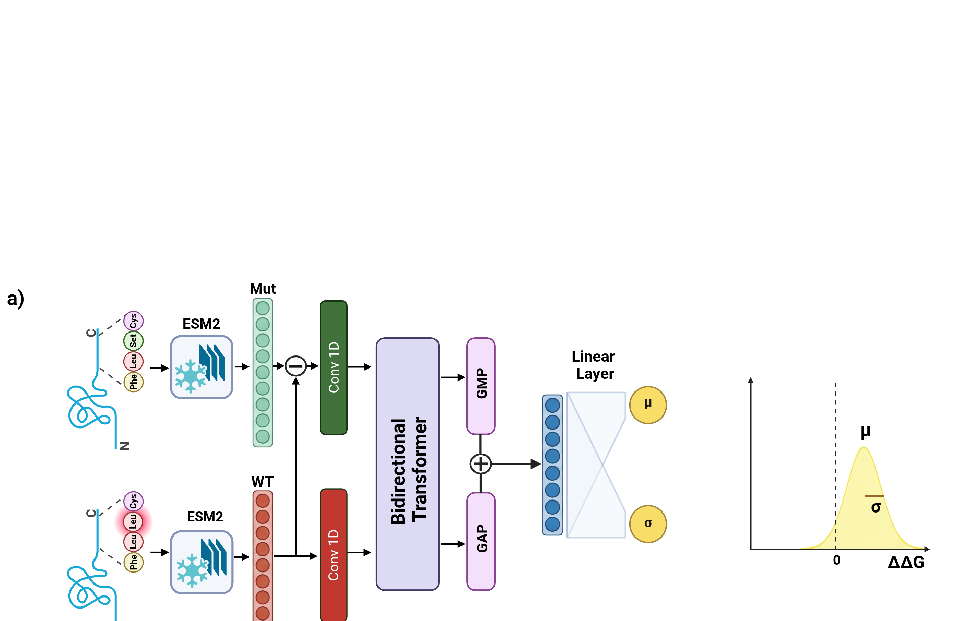
\includegraphics[width=\linewidth,height=0.75\textheight,keepaspectratio]{figures/architecture.pdf}
    \end{column}
    \begin{column}{0.35\textwidth}
      \textbf{Antisymmetric mean}
      \[
        \mu(A,B)=-\mu(B,A).
      \]
      \textbf{Symmetric scale}
      \[
        \sigma(A,B)=\sigma(B,A).
      \]
      {\small Positive scale modulates interval width.}
    \end{column}
  \end{columns}
  \sources{Manuscript, Figure 1a and Section 2.3.}
  \note{Tempo: 1 minuto e mezzo. Mostra i due output: media e scala positiva. L'inversione del verso cambia il segno della media e mantiene la scala. Il training usa una likelihood gaussiana, ma la calibrazione conformal non richiede residui gaussiani. Non presentare sigma come l'errore esatto della singola mutazione.}
\end{frame}

% 08 --- 1:30
\begin{frame}{Protein-weighted CV+ calibration}
  Each calibration mutation uses a model that excluded its entire outer fold.
  \[
    r_i=\frac{|y_i-\mu_{k(i)}(x_i)|}{\sigma_{k(i)}(x_i)}.
  \]
  For a new mutation, preserve the score--model pairing:
  \[
    \ell_i(x)=\mu_{k(i)}(x)-r_i\sigma_{k(i)}(x),\quad
    u_i(x)=\mu_{k(i)}(x)+r_i\sigma_{k(i)}(x).
  \]
  \[
    C_{1-\alpha}(x)=
    [Q^w_\alpha(\ell_i(x)),\;Q^w_{1-\alpha}(u_i(x))].
  \]
  \sources{Manuscript Section 2.6. Empirical weighted-quantile convention. Standard CV+ uses unnormalized absolute residuals with the same models and weights.}
  \note{Tempo: 1 minuto e mezzo. La scala normalizza il residuo della mutazione di calibrazione e lo riscalibra per la mutazione nuova. Ogni residuo rimane associato al modello che lo ha prodotto. La predizione puntuale e la mediana dei cinque modelli, ma l'intervallo non deriva semplicemente da questa mediana piu o meno un margine globale. Non confondere il livello nominale con il limite inferiore teorico della copertura.}
\end{frame}

% 09 --- 1:00
\begin{frame}{Training and external evaluation}
  \begin{center}
    \begin{tabular}{lrrl}
      \toprule
      Dataset & Mutations & Proteins & Role \\
      \midrule
      S2450 & 2,450 & 115 & Training / calibration \\
      S669L & 669 & 87 & External evaluation \\
      S461L & 461 & 46 & Curated, overlapping subset \\
      \bottomrule
    \end{tabular}
  \end{center}
  \medskip
  \begin{itemize}
    \item Five outer folds separate proteins using a 25\% sequence-identity threshold.
    \item Epoch selection excludes the outer fold; refitting uses the other four folds.
    \item External targets enter evaluation only.
  \end{itemize}
  \sources{Manuscript, Sections 2.2 and 2.5. S461L does not provide independent replication.}
  \note{Tempo: 1 minuto. Presenta S669L come benchmark principale del talk. S2450 esclude anche le proteine oltre il 25 percento di identita con il benchmark S669. Descrivi brevemente la selezione interna delle epoche e il successivo refit: il fold esterno non entra ne nella selezione ne nel fitting. S461L e un sottoinsieme curato, non un secondo esperimento indipendente.}
\end{frame}

% 10 --- 1:00
\begin{frame}{External point-prediction performance}
  \begin{center}
    \begin{tabular}{lrrrr}
      \toprule
      Dataset & Pearson $r$ & Spearman $\rho$ & MAE & MSE \\
      \midrule
      S669L & 0.53 & 0.55 & 0.99 & 2.03 \\
      S461L & 0.70 & 0.68 & 0.74 & 0.97 \\
      \bottomrule
    \end{tabular}
  \end{center}
  \medskip
  MAE in \units; MSE in $(\units)^2$.
  \medskip
  All test mutations contribute equally to these summaries.
  \takeaway{Point accuracy provides context for evaluating interval usefulness.}
  \sources{Manuscript, Table 1. Median of five fold-specific predictions.}
  \note{Tempo: 1 minuto. Non presentare questo risultato come una vittoria sulla performance di JanusDDG o di tutti i competitor. Le prestazioni puntuali forniscono il contesto: l'obiettivo centrale del lavoro e integrare incertezza interpretabile. I numeri storici dei competitor provengono da benchmark pubblicati e non da un confronto rifatto in questo studio.}
\end{frame}

% 11 --- 1:30
\begin{frame}{Mutation and protein coverage}
  \begin{columns}[T,onlytextwidth]
    \begin{column}{0.47\textwidth}
      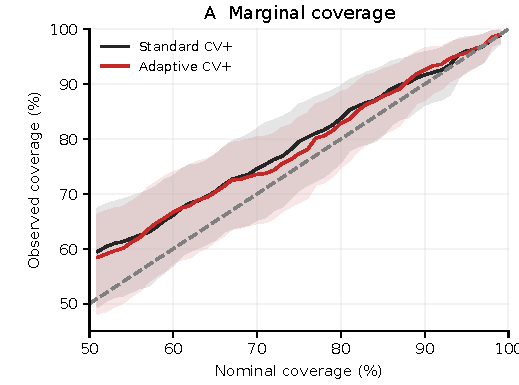
\includegraphics[width=\linewidth]{figures/coverage_curve.pdf}
    \end{column}
    \begin{column}{0.50\textwidth}
      \textbf{S669L, 90\% nominal level}
      \medskip
      {\small
      \begin{tabular}{lrr}
        \toprule
        Coverage & Standard & Adaptive \\
        \midrule
        Mutations & 91.63\% & 92.53\% \\
        Proteins & 86.76\% & 86.87\% \\
        \bottomrule
      \end{tabular}}
    \end{column}
  \end{columns}
  \takeaway{Protein-averaged coverage: approximately 87\%.}
  \sources{S669L. Figure 2a and Table 3. Curve and pointwise bootstrap bands weight mutations equally.}
  \note{Tempo: 1 minuto e mezzo. Questa e una slide centrale. La pesatura durante la calibrazione e diversa dalla pesatura della metrica di valutazione. La curva mostra copertura sulle mutazioni; la tabella esplicita il target con uguale peso delle proteine. Non dire che il 90 percento nominale e stato raggiunto sul target protein-balanced: qui osserviamo circa 87 percento. Le bande bootstrap sono puntuali e mantengono fissi i modelli.}
\end{frame}

% 12 --- 1:30
\begin{frame}{Adaptive intervals redistribute width}
  \begin{columns}[T,onlytextwidth]
    \begin{column}{0.49\textwidth}
      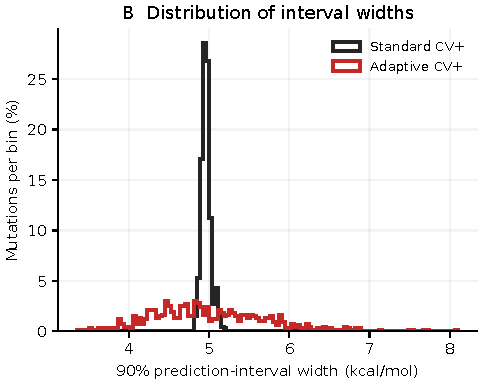
\includegraphics[width=\linewidth]{figures/width_distribution.pdf}
    \end{column}
    \begin{column}{0.49\textwidth}
      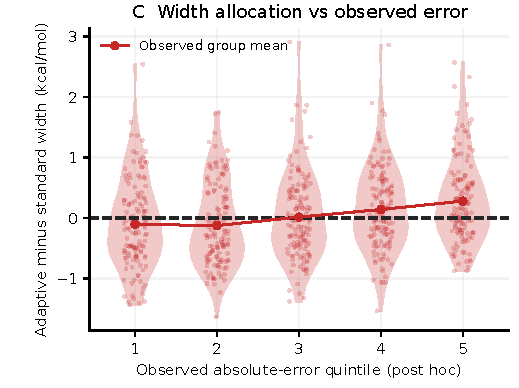
\includegraphics[width=\linewidth]{figures/width_allocation.pdf}
    \end{column}
  \end{columns}
  \medskip
  {\small Mean full width: \textbf{4.964} standard vs \textbf{5.004} adaptive \units.}
  \sources{S669L, 90\% nominal. Figure 2b--c and Table 3. Error quintiles are post-hoc diagnostics.}
  \note{Tempo: 1 minuto e mezzo. Parti dalla distribuzione delle ampiezze: la versione standard non ha ampiezza perfettamente costante perche CV+ combina modelli diversi. La versione adattiva assegna intervalli piu diversi alle mutazioni mantenendo una media simile. A destra, la differenza adattivo meno standard cresce mediamente dal quintile a basso errore a quello ad alto errore. I gruppi usano gli errori osservati solo dopo la valutazione, non per selezionare prospetticamente le mutazioni.}
\end{frame}

% 13 --- 1:00
\begin{frame}{Learned scale and uncertainty groups}
  \begin{columns}[T,onlytextwidth]
    \begin{column}{0.49\textwidth}
      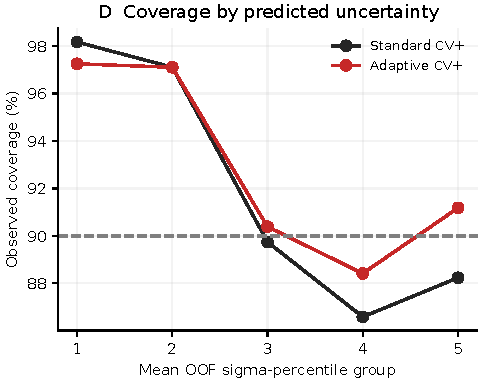
\includegraphics[width=\linewidth]{figures/uncertainty_groups.pdf}
    \end{column}
    \begin{column}{0.47\textwidth}
      \textbf{Error association}\par
      Spearman $\rho=0.22$.
      \par\medskip
      \textbf{Coverage dispersion}\par
      Standard: 4.75 pp.\par
      Adaptive: 3.63 pp.
    \end{column}
  \end{columns}
  \sources{S669L. Figure 2d and Table 3. Fixed OOF scale-percentile groups. No subgroup-coverage guarantee.}
  \note{Tempo: 1 minuto. Il rango di incertezza e la media dei percentili di sigma rispetto al fold di calibrazione di ciascun modello. La correlazione 0.22 e moderata: sigma non misura precisamente l'errore individuale. La dispersione e la deviazione standard di popolazione delle cinque coperture, in punti percentuali. Il risultato descrive una riduzione della variabilita osservata, non una garanzia di copertura condizionata al gruppo.}
\end{frame}

% 14 --- 2:00
\begin{frame}{Sign-call frequency and accuracy}
  Stabilizing if $L_i>0$; destabilizing if $U_i<0$.
  Intervals touching zero yield no call.
  \medskip
  \begin{center}
    {\small
    \begin{tabular}{rrrrr}
      \toprule
      Nominal & Calls & Call rate & Correct / called & Proteins reached \\
      \midrule
      50\% & 229 & 34.23\% & 217/229 (94.76\%) & 46/87 \\
      60\% & 171 & 25.56\% & 167/171 (97.66\%) & 37/87 \\
      70\% & 104 & 15.55\% & 103/104 (99.04\%) & 21/87 \\
      90\% & 4 & 0.60\% & 4/4 (100\%) & 2/87 \\
      \bottomrule
    \end{tabular}}
  \end{center}
  \takeaway{Higher nominal levels yield fewer directional calls.}
  \sources{S669L, adaptive CV+, manuscript Figure 4 and Table 5. Empirical accuracy among selected calls is distinct from nominal interval coverage. All four 90\% calls are destabilizing.}
  \note{Tempo: 2 minuti. Mostra il compromesso operativo tra numero di decisioni e accuratezza osservata. Non confondere un intervallo nominale del 50 percento con una probabilita del 50 percento che il segno sia corretto. Il 100 percento al 90 percento nominale deriva da sole quattro chiamate: non e evidenza di certezza. Le chiamate sono prevalentemente destabilizzanti e vanno interpretate nella composizione di questo benchmark. Le proteine raggiunte hanno almeno una mutazione chiamata, non tutte le mutazioni risolte.}
\end{frame}

% 15 --- 1:00
\begin{frame}{Conclusions}
  \begin{itemize}
    \item Protein-weighted calibration gives each observed protein equal influence.
    \item Adaptive CV+ redistributes interval width with a similar mean width.
    \item Zero-excluding intervals support selective sign decisions.
  \end{itemize}
  \medskip
  \textbf{Scope of the evidence}\par
  \smallskip
  Protein-averaged coverage remains below 90\% on S669L. Benchmark composition affects observed coverage.
  \takeaway{Uncertainty evaluation complements point-prediction performance.}
  \note{Tempo: 1 minuto. Riporta il messaggio principale: la valutazione dell'incertezza affronta un problema complementare alla MAE. Chiudi mantenendo visibile il limite sul target protein-balanced. La teoria richiede ipotesi specifiche di campionamento e fitting; non offre una garanzia per ogni singola proteina o per l'accuratezza delle sole chiamate. Se c'e tempo o una domanda, usa le slide di riserva.}
\end{frame}

\appendix
\backuptrue

% Backup A
\begin{frame}{Backup: the curated S461L subset}
  \textbf{90\% nominal level}
  \medskip
  \begin{center}
    \begin{tabular}{lrr}
      \toprule
      S461L metric & Standard & Adaptive \\
      \midrule
      Mutation coverage & 97.61\% & 98.05\% \\
      Protein-averaged coverage & 96.56\% & 93.85\% \\
      Mean full width (\units) & 4.965 & 4.967 \\
      Mean interval score (\units) & 5.188 & 5.109 \\
      \bottomrule
    \end{tabular}
  \end{center}
  \takeaway{Benchmark curation changes observed calibration behavior.}
  \sources{Manuscript, Table 3. S461L overlaps S669L and does not provide independent replication.}
  \note{Slide di riserva. S461L e piu conservativo: non raccontare questo come una seconda conferma indipendente del 90 percento. La composizione del benchmark cambia i risultati e l'adattivita non migliora sistematicamente ogni metrica, inclusa la media per proteina.}
\end{frame}

% Backup B
\begin{frame}{Backup: calibration of a one-hot baseline}
  \textbf{S669L, 90\% nominal level}
  \medskip
  \begin{center}
    {\small
    \begin{tabular}{lrr}
      \toprule
      Adaptive intervals & ProbJanusDDG & One-hot baseline \\
      \midrule
      Pearson $r$ & 0.53 & 0.33 \\
      MAE (\units) & 0.99 & 1.23 \\
      Mutation coverage & 92.53\% & 90.28\% \\
      Protein-averaged coverage & 86.87\% & 86.41\% \\
      Mean full width (\units) & 5.004 & 5.84 \\
      \bottomrule
    \end{tabular}}
  \end{center}
  \takeaway{Lower point accuracy coincides with wider intervals.}
  \sources{Manuscript, Tables 1, 3 and 4, Section 3.3.5. Same training and calibration protocol, different architecture and representation.}
  \note{Slide di riserva. Il confronto cambia sia architettura sia rappresentazione: non attribuire la differenza solo agli embedding. La calibrazione opera su entrambi i predittori; la qualita del modello determina quanto informativi possono essere gli intervalli. Le coperture per proteina restano inferiori al nominale in entrambi.}
\end{frame}

% Backup C
\begin{frame}{Backup: coverage assumptions}
  \begin{itemize}
    \item Independent protein clusters with aligned within-protein sampling.
    \item Data-independent fold allocation and fitting outside each calibration fold.
  \end{itemize}
  \medskip
  For the empirical weighted rule, the draft Appendix gives:
  \[
    \Pr\{Y_*\in C_{1-\alpha}(X_*)\}
    \geq 1-2\alpha-\frac{2(1-\alpha)K}{P+K}.
  \]
  \medskip
  Marginal bound for the protein-balanced target. Homology-based folds require separate justification.
  \sources{Draft theoretical Appendix developed alongside the manuscript. The bound is not an assertion of exact nominal coverage or selected-sign accuracy.}
  \note{Slide di riserva. Da usare solo se l'appendice teorica e inclusa nella versione definitiva del paper. Il modello gerarchico assume proteine indipendenti, una legge delle mutazioni che non dipende dalla dimensione osservata del cluster dopo aver condizionato sulla proteina, e allineamento del test al target. I fold devono essere indipendenti dai dati per questo risultato. Queste ipotesi non sono automaticamente soddisfatte da fold basati sull'omologia. Il limite e finito-campione, debole, e non equivale alla copertura nominale del 90 percento.}
\end{frame}

% Backup D
\begin{frame}{Selected references}
  \small
  \textbf{Barducci et al. (2026).} JanusDDG.\par
  \textit{Communications Biology} 9, 494.\par
  \href{https://doi.org/10.1038/s42003-026-09632-9}{doi:10.1038/s42003-026-09632-9}
  \par\medskip
  \textbf{Angelopoulos, Barber and Bates (2026).}\par
  \textit{Theoretical Foundations of Conformal Prediction}.\par
  \href{https://arxiv.org/abs/2411.11824}{arXiv:2411.11824v5}
  \par\medskip
  \textbf{Wang et al. (2022).} BayeStab.\par
  \textit{Protein Science} 31, e4467.
  \par\medskip
  \textbf{Sapozhnikov et al. (2023).} FoldX uncertainty modeling.\par
  \textit{BMC Bioinformatics} 24, 426.\par
  \href{https://doi.org/10.1186/s12859-023-05537-0}{doi:10.1186/s12859-023-05537-0}
  \note{Slide di riserva per i riferimenti. Le figure e i valori di ProbJanusDDG provengono dal manoscritto allegato, versione prob\_janus (6).pdf. Il libro e la versione pre-publication allegata del 6 marzo 2026.}
\end{frame}

\end{document}
